\chapter{Introduction}
\label{c:intro}
Smart glasses provide always-available displays and offer the opportunity for instantly available information and pervasive gaming experiences. 
Compared to game consoles and mobile gaming devices, smart glasses do not have touchscreens and currently do not support handheld controllers specifically designed for gaming.
Current smart glasses, such as Google Glass and the Epson Moverio, support input via voice, touchpads, cameras, gyroscopes, accelerometers, and GPS.
Games designed specifically for Google Glass \cite{MiniGames} utilize these sensors as game control. 
For example, ``Clay Shooter'' utilizes the user's voice to trigger a shotgun, and ``Shape Splitter'' detects in-air gestures via the built-in cameras. 
For the Epson Moverio glasses, wired trackpads are used as handheld inputs.


 \begin{figure}[!t]
  \centering
  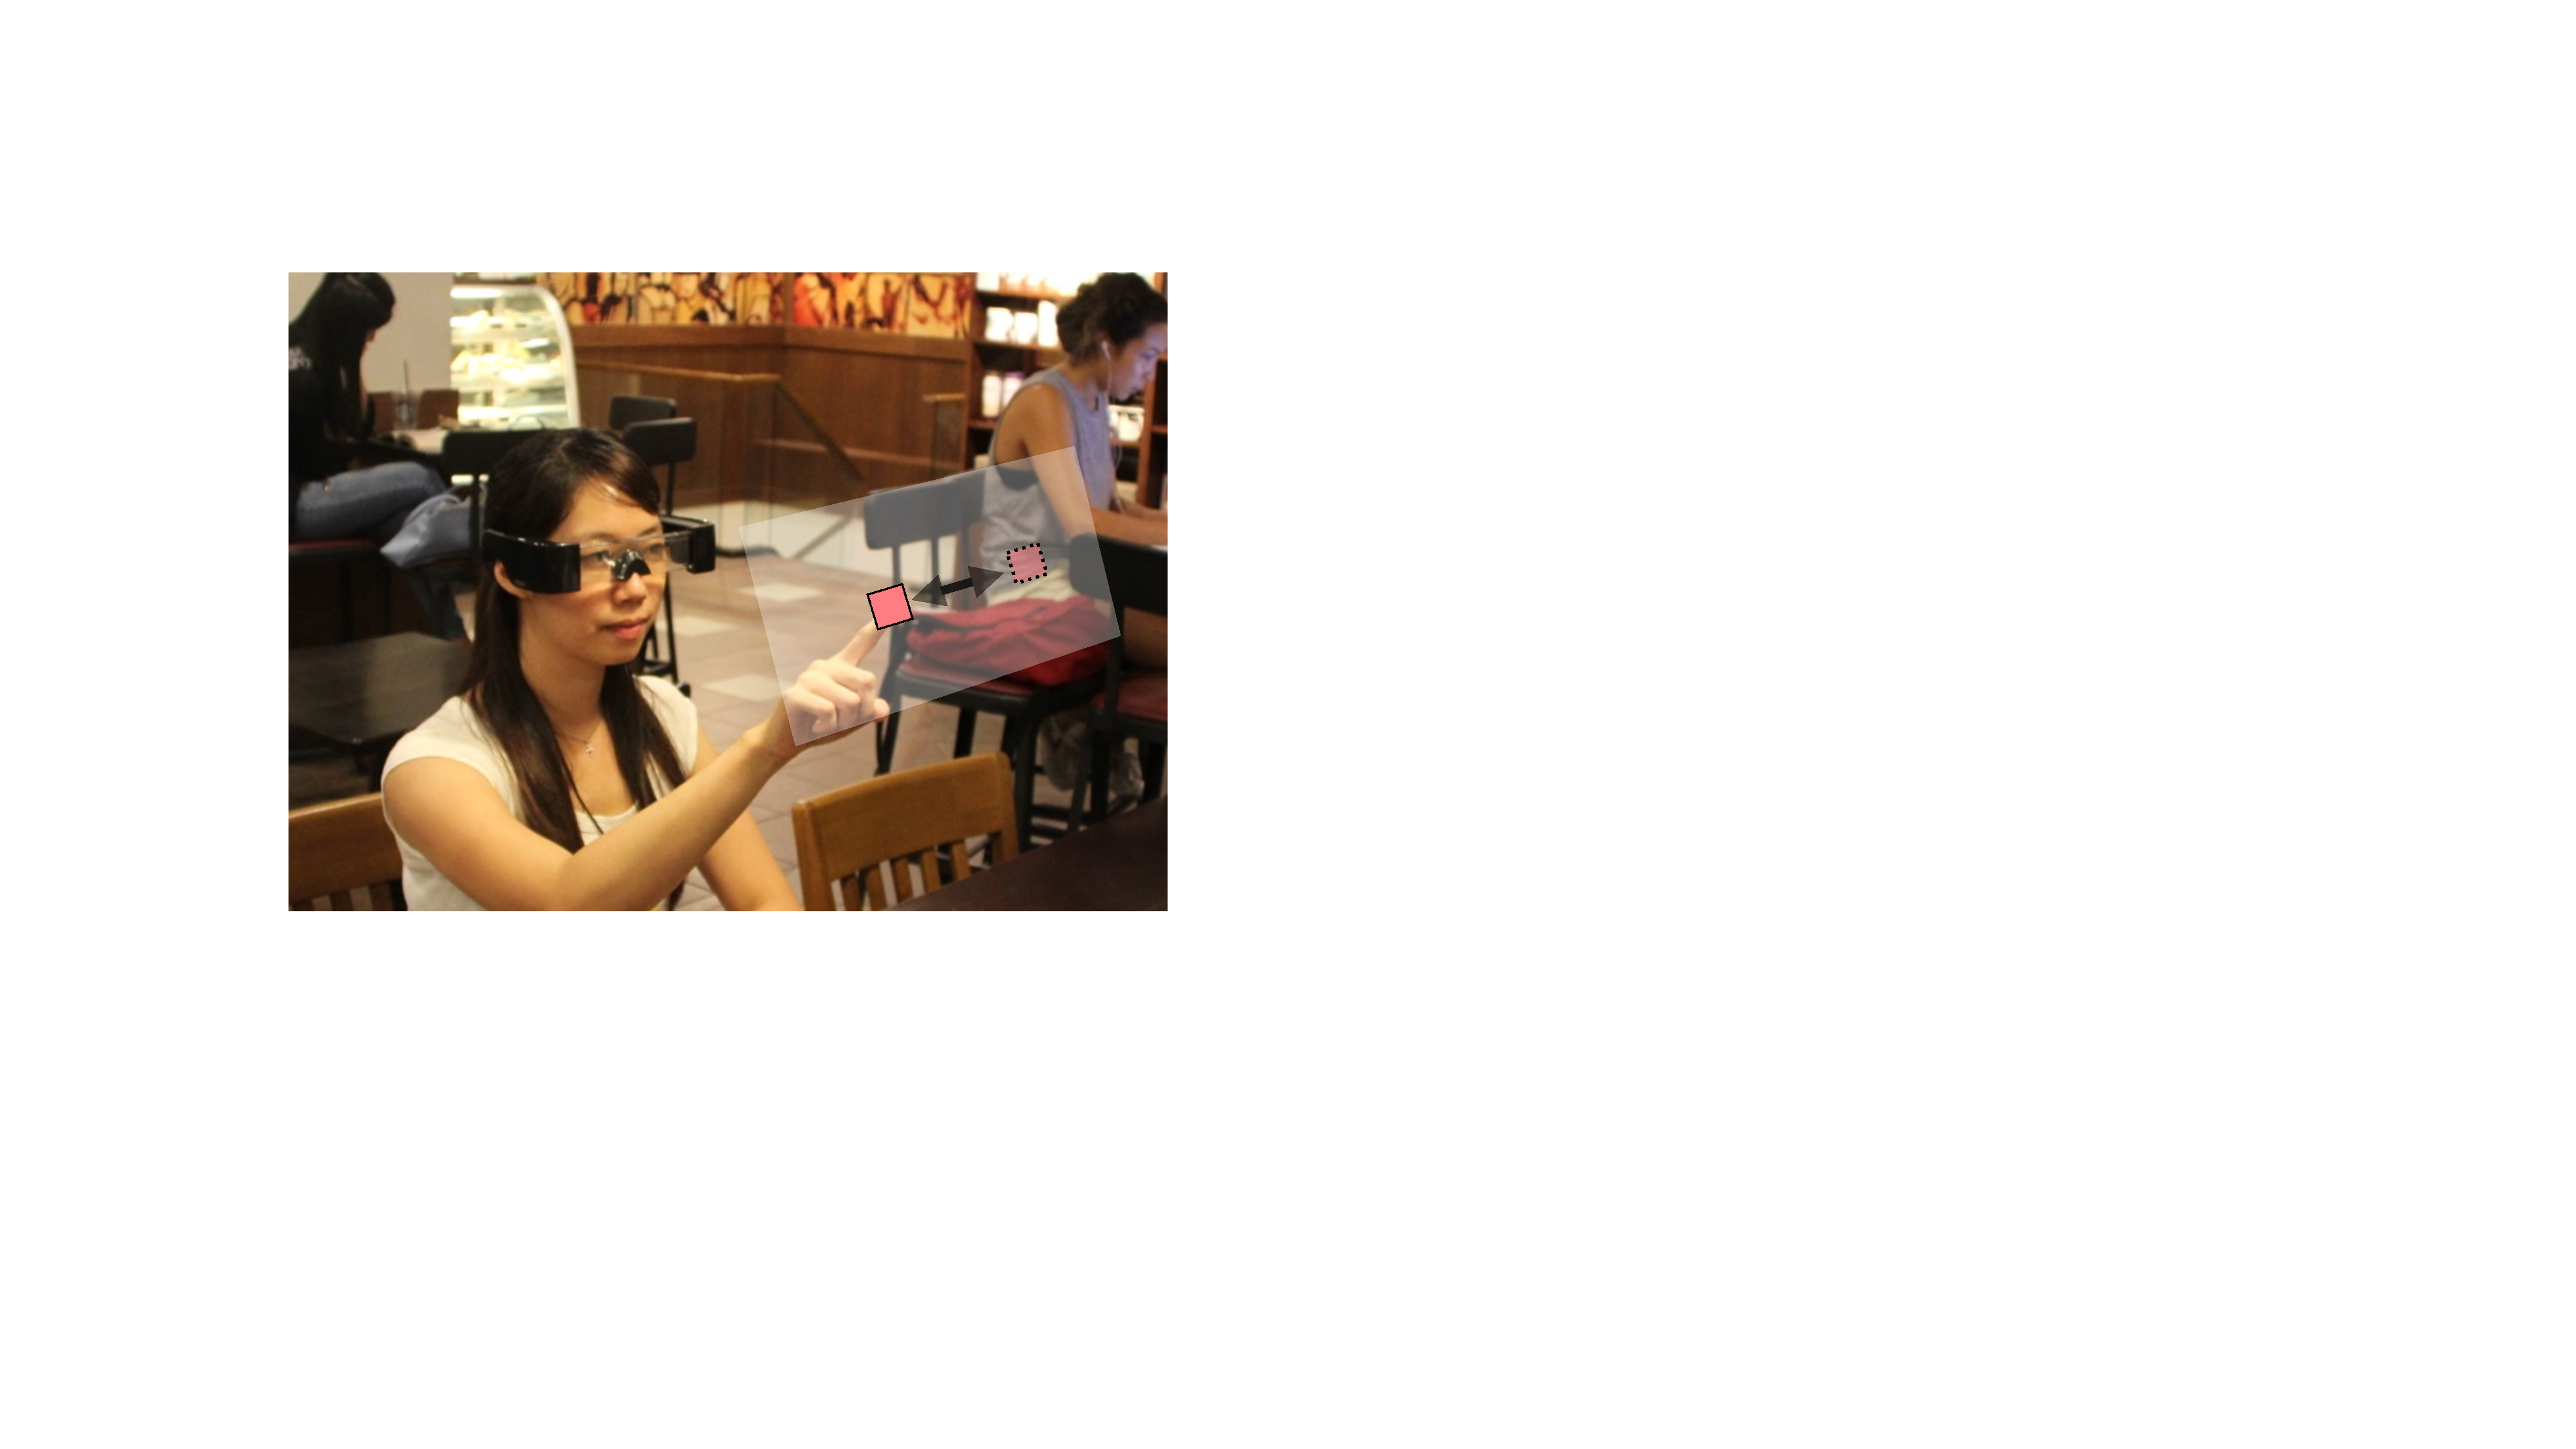
\includegraphics[width=1\columnwidth]{Figures/TopFigure2.pdf}
  \caption{A study participant performing an in-air gesture to drag an object seen through the immersive smart glasses in a public coffee shop.}
  \label{fig:TopFigure}
  \end{figure} 

To better inform the interaction design of games for smart glasses, we aimed to explore the design space without being constrained by the capabilities of current sensors. We used the guessability study methodology \cite{Wobbrock:2005:MGS:1056808.1057043}, and presented the \emph{effects} of game controls to the participants in a real-world, public environment. We then elicited what the participants felt was the most appropriate \emph{causes} to invoke the corresponding effects. 

    \begin{figure}[!b]
  \centering
  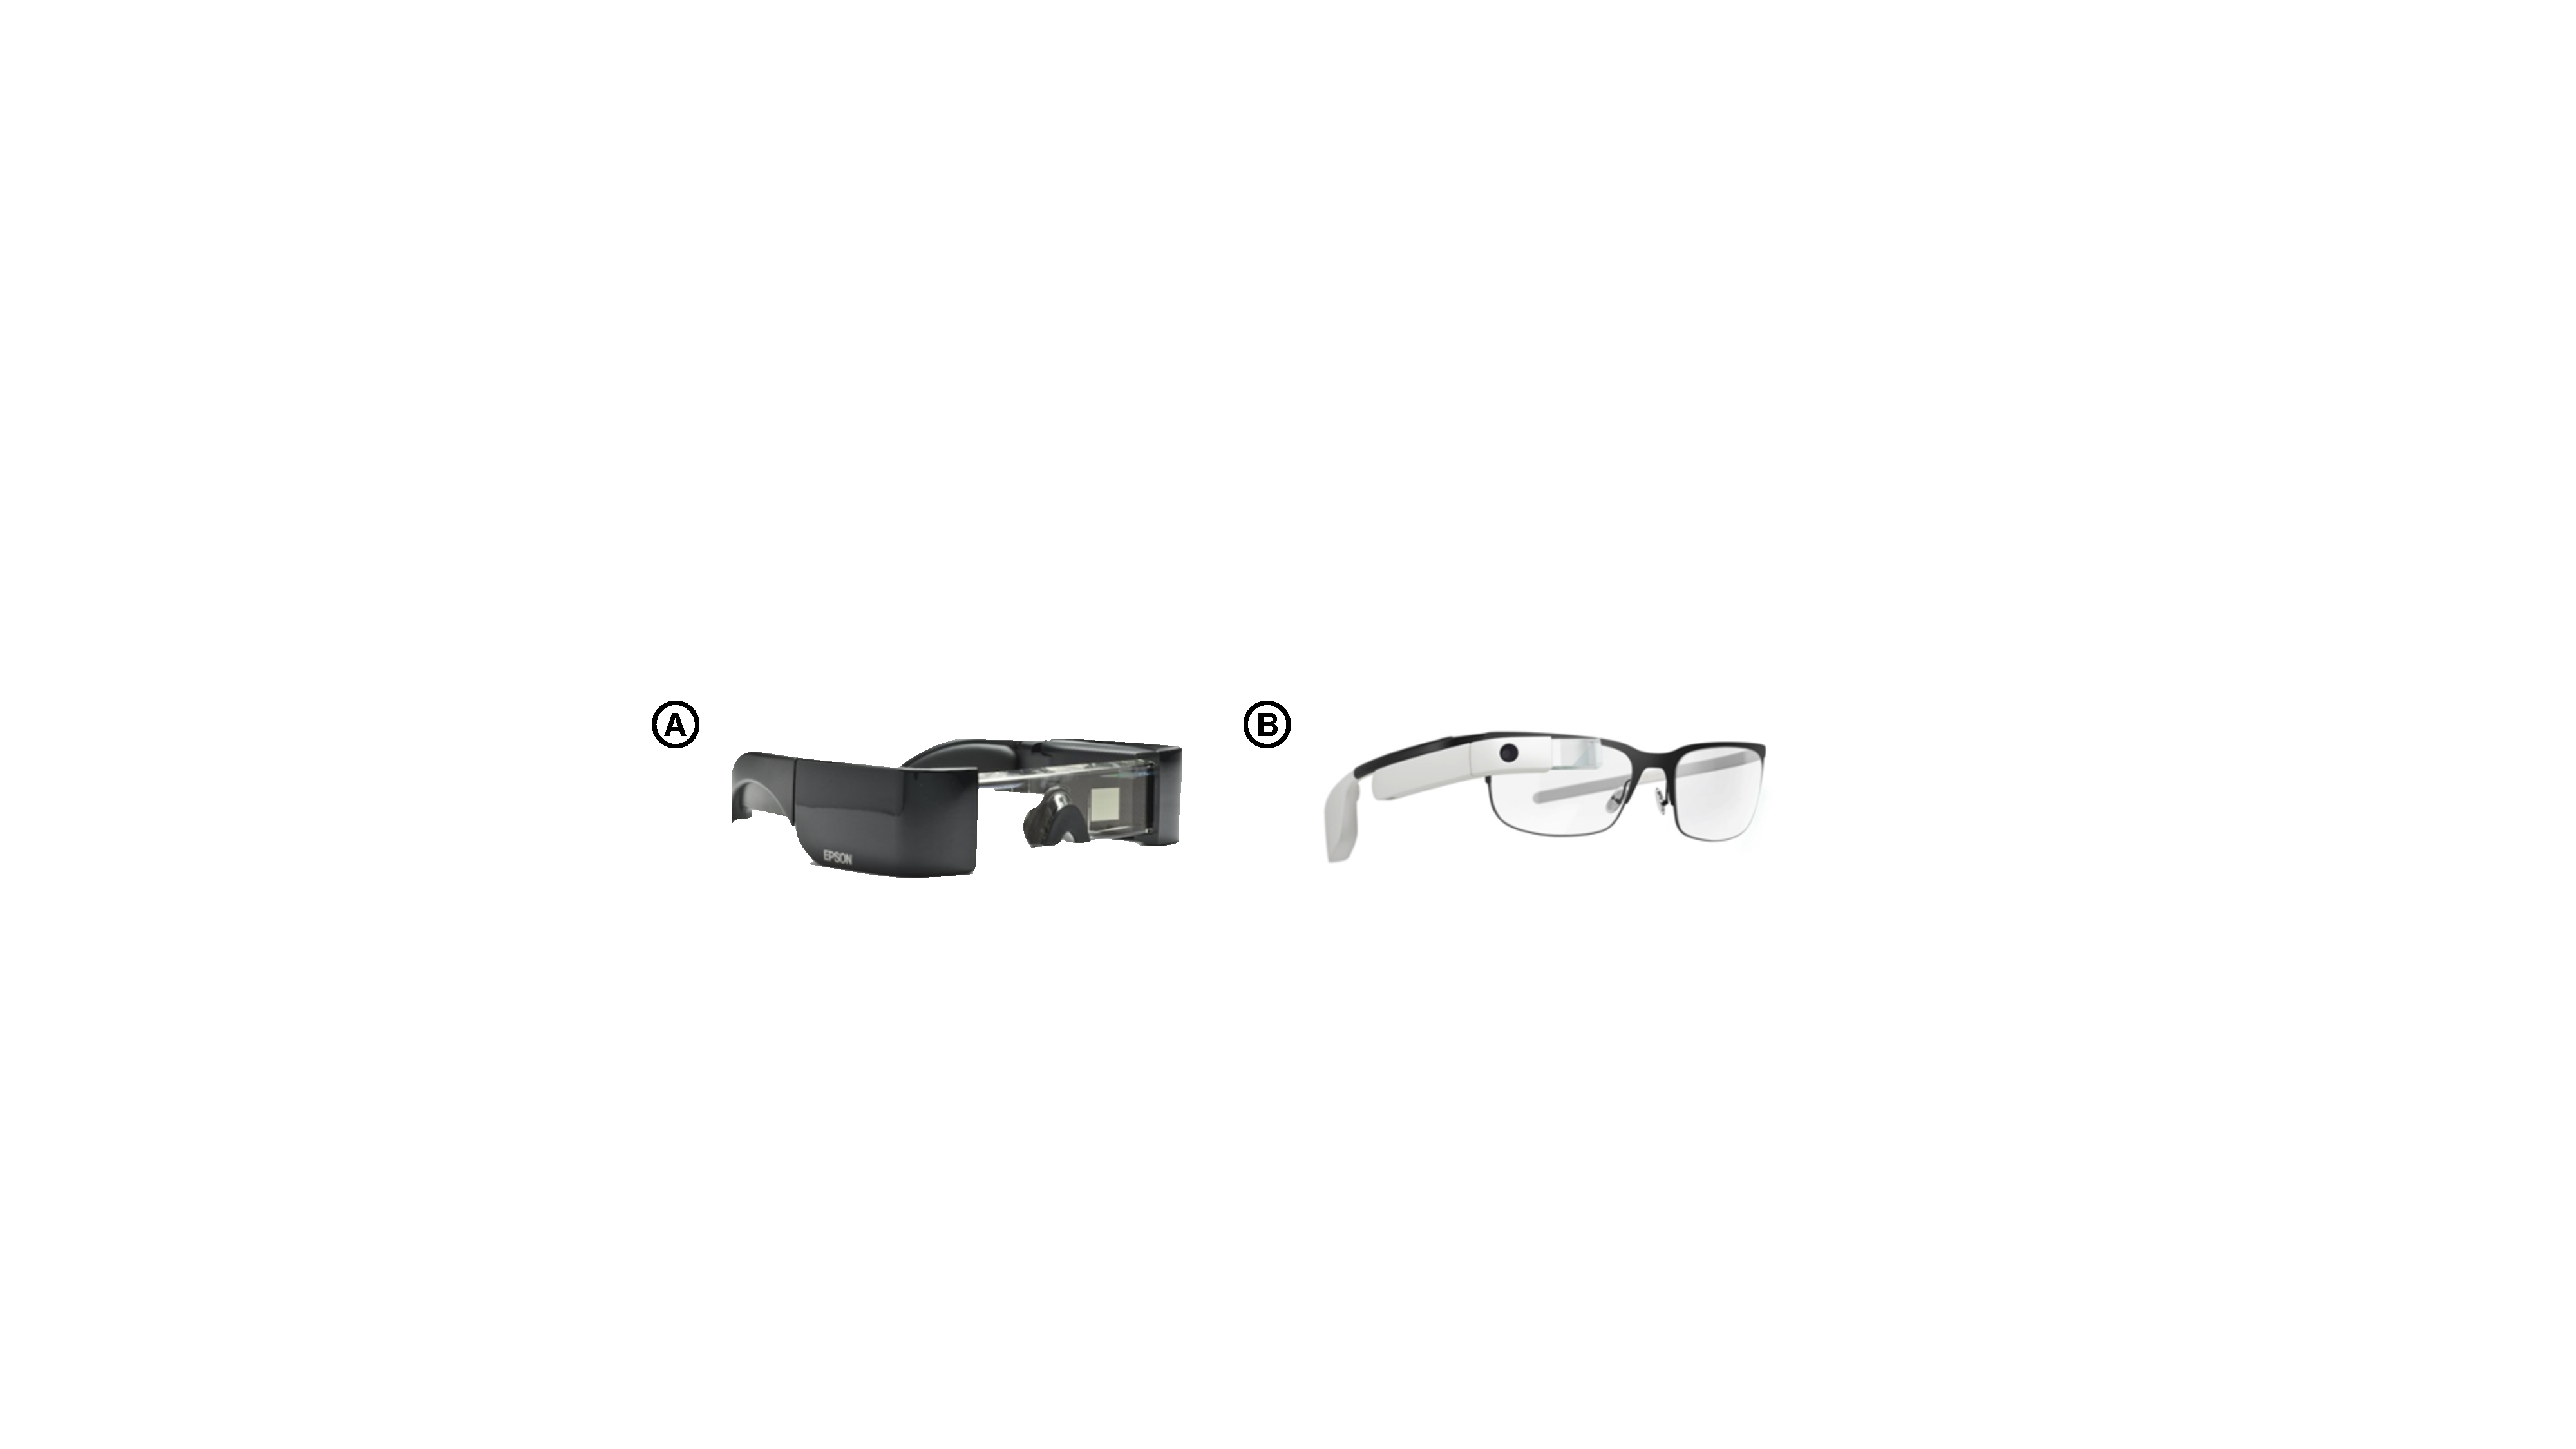
\includegraphics[width=1\columnwidth]{Figures/Glasses.pdf}
  \caption{(A) Epson Moverio, (B) Google Glass.}
  \label{fig:Glasses}
  \end{figure}

For input tasks, we analyzed 90 popular games to identify the game controls used by more than one game, which resulted in a set of 17 tasks. We also explored the form factors of smart glasses displays, and included both types in the study: 1) \emph{immersive}, with display content spanning the user's field of view (e.g. Epson and Sony's smart glasses), and 2) \emph{off-to-the-side}, with display content in the corners of the user's field of view (e.g. Google Glass).

In order to compare different types of interaction while keeping the experiment tractable, we grouped the different types of input into the following 3 classes:
\begin{itemize}
  \item \emph{handheld}: input types that make use of handheld controllers, such as smartphones and the wired trackpads used by Sony's SmartEyeglass and Epson's Moverio glasses.
  \item \emph{touch}: non-handheld touch input, such as gesturing and tapping on body surfaces, and touch-sensing wearable devices (e.g. smart rings, watches, and glasses). These provide tactile feedback.
  \item \emph{non-touch}: non-handheld, non-touch input, such as in-air gestures, head/body movement, and voice recognition. These do not have tactile feedback.
\end{itemize}
 


We recruited 24 participants and asked them to wear the two form factors of smart glasses in a coffee shop. On-screen instructions prompted participants to perform each of the 17 common game control tasks using the 3 classes of input types. For each game control task, form factor, and input type, participants first explored all possible interactions they could think of, then reported the one they most preferred. After completing the 3 types of interactions for that task and form factor, they then rated their preferences for 3 interactions.  Overall, each participant reported 102 interactions, for a total of 2448. 

We collected quantitative and qualitative data through video analysis, preference ratings, and interviews. 
Our key observations are as follows:
\begin{itemize}
  \item Participants significantly preferred non-handheld, non-touch interactions over handheld interactions (3.81  vs 3.68 on a 5-point Likert scale, $p$\textless 0.01).
  \item For touch input without using handheld devices, users preferred interacting with their body surface over wearable devices (80\% vs 20\%), and the most frequently used body surface was the palm (51\%).
  \item Participants preferred interactions that are more subtle due to concerns with social acceptance. Also, participants preferred using in-air gestures in front of the torso than in front of the face (63\% vs 37\%), even though those gestures were reported to be less intuitive and less precise.
  \item There is a significant mismatch between participants' preferred input methods and those supported by the current smart glasses. For example, less than 2\% of the participants used voice and less than 2\% of the participants used touch input on the smart glasses -- which are Google Glass' two primary input methods. In addition, current cameras can only detect in-air gestures in front of users' faces, missing most 63\% of the gestures performed.
\end{itemize}

 
The contribution of this paper are as follows:
(1) the first quantitative and qualitative characterization of user-defined input for games on smart glasses, including a taxonomy, 
(2) set of user-defined input for common game tasks, which is reflective of user behavior.
(3) insight into users' mental models when playing smart glasses games in a public space, and an understanding of implications for mobile input technology and user interface design.
Our results will help designers create better smart glasses experience informed by user behavior.
